\chapter{Codifica senza distorsione}

\thispagestyle{empty}

Consideriamo la seguente procedura:
\begin{enumerate}

    \item La BS stima il canale di uplink, lo codifica con un codificatore
        adeguato e invia la versione codificata allo UT.

    \item Lo UT stima il canale di downlink e, utilizzando anche il messaggio
        ricevuto al punto 1, codifica il canale e lo trasmette alla BS.

    \item La BS utilizza il canale di UL stimato al punto 1, la sua versione
        codificata del punto 1 e il messaggio ricevuto al punto 2 per stimare
        il canale.

\end{enumerate}
Le codifiche effettuate ai punti 1 e 2 sono con parole di codice di lunghezza
variabile, pertanto il tasso di comunicazione nei punti 1 e 2 è variabile. Sia
\(b_\mathrm{F}\) il numero medio di bit usati per la codifica al punto 1 e
\(b_\mathrm{B}\) il numero medio di bit usati per la codifica al punto 2.

Detto quindi \(b_\mathrm{F}\) il numero di bit trasmessi in feedforward, ovvero
dalla BS allo UT, e detto \(b_\mathrm{B}\) il numero di bit trasmessi come
feedback, dallo UT alla BS, definiamo
\[
    B = b_\mathrm{F} + b_\mathrm{B}
\]
il numero totale di bit scambiati tra BS e UT.

Nella procedura a tasso variabile, illustrata in seguito, imponiamo
\(b_\mathrm{F} = 0\), ovvero nessun bit viene inviato dalla BS allo UT in
feedforward. In particolare, permettiamo al numero di bit di feedback
\(b_\mathrm{B}\) di variare, pertanto la segnalazione di feedback ha un tasso
variabile.

Anzitutto, modelliamo lo scenario considerato come una codifica di sorgente di
due sorgenti correlate (i canali di UL e DL, in questo caso). Quindi,
dimostreremo che la presenza di una segnalazione di feedforward da parte della
BS non contribuisce a ridurre il tasso medio della segnalazione di feedback,
risultando quindi superflua al fine di ridurre l'overhead complessivo. Infine,
proponiamo una procedura con approccio feedback-only a tasso variabile, basata
sull'entropia condizionale del canale di DL condizionata al canale di UL.

\section{Codifica di sorgenti correlate}

Dal teorema di Shannon sulla codifica di sorgente
\cite{10.1002/j.1538-7305.1948.tb01338.x} è noto che per codificare una
sorgente \(X\), un tasso \(R > \entropy{X}\) è sufficiente. Consideriamo ora
due sorgenti correlate \((X,Y) \sim p(x, y)\). In questo caso, un tasso pari a
\(\entropy{X,Y}\) è sufficiente per codificarle congiuntamente. Supponiamo che
al ricevitore si desideri ricostruire \(X\) e \(Y\) separatamente. Si vede
facilmente che un tasso \(R = R_X + R_Y > \entropy{X} + \entropy{Y}\) è
sufficiente. Tuttavia, Slepian e Wolf \cite{1055037} hanno dimostrato che un
tasso totale pari a \(R = \entropy{X,Y}\) è sufficiente anche per codificare
separatamente le due sorgenti correlate.

Riportiamo nel seguito il teorema di Slepian-Wolf
\cite{10.1002/047174882X.ch15}. In Figura~\ref{fig:sw-configuration} è
illustrata la situazione considerata.

\begin{figure}[ht]
    \centering
    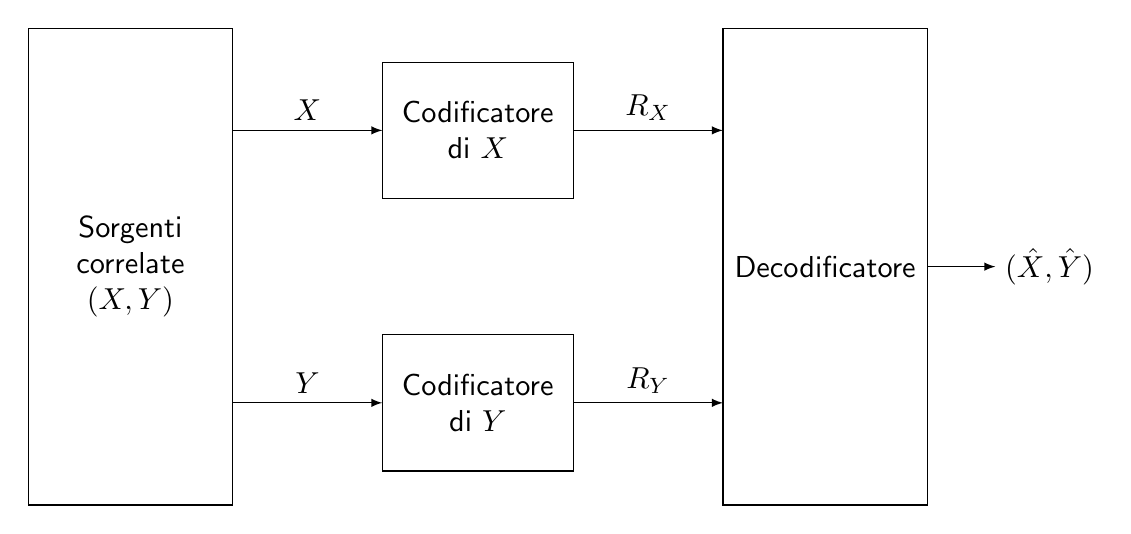
\begin{tikzpicture}[scale=0.865,>=latex]
    \tikzstyle{every node}=[font=\fontsize{11}{13}\sffamily]

    \draw (0,0) rectangle (3,7)
    node[midway,align=center]{Sorgenti \\ correlate \\ \((X,Y)\)};

    \draw[->] (3,5.5) -- (5.2,5.5)
    node[above,midway]{\(X\)};

    \draw[->] (3,1.5) -- (5.2,1.5)
    node[above,midway]{\(Y\)};

    \draw (5.2,4.5) rectangle (8,6.5)
    node[midway,align=center]{Codificatore \\ di \(X\)};

    \draw (5.2,0.5) rectangle (8,2.5)
    node[midway,align=center]{Codificatore \\ di \(Y\)};

    \draw[->] (8,5.5) -- (10.2,5.5)
    node[above,midway]{\(R_X\)};

    \draw[->] (8,1.5) -- (10.2,1.5)
    node[above,midway]{\(R_Y\)};

    \draw (10.2,0) rectangle (13.2,7)
    node[midway]{Decodificatore};

    \draw[->] (13.2,3.5) -- (14.2,3.5)
    node[right]{\((\hat{X},\hat{Y})\)};
\end{tikzpicture}

    \caption{Configurazione per la codifica di sorgente Slepian-Wolf.}
    \label{fig:sw-configuration}
\end{figure}

\begin{thm}[Slepian-Wolf \textnormal{\cite{10.1002/047174882X.ch15}}]
    \label{thm:sw}

    Sia \((X_1,Y_1),(X_2,Y_2),\dots\) una sequenza di variabili aleatorie
    congiunte, indipendenti e identicamente distribuite tali che la generica
    coppia \((X,Y) \sim p(x, y)\).\\
    Per il problema della codifica di sorgenti distribuite per la sorgente
    \((X,Y)\), la regione di tasso raggiungibile è data da
    \begin{alignat}{1}
        R_X &\ge \entropy{X \vert Y}, \label{eq:SW1} \\
        R_Y &\ge \entropy{Y \vert X}, \label{eq:SW2} \\
        R_X + R_Y &\ge \entropy{X,Y}. \label{eq:SWsum}
    \end{alignat}
\end{thm}

La Figura~\ref{fig:sw-rate-region} mostra la regione descritta dal
Teorema~\ref{thm:sw}.

\begin{figure}[ht]
    \centering
    \begin{tikzpicture}[>=latex]
    %\tikzstyle{every node}=[font=\fontsize{11}{13}\sffamily]

    \draw[->] (0,0) -- (8,0)
    node[right]{\(R_X\)};

    \draw[->] (0,0) -- (0,6)
    node[above]{\(R_Y\)};

    \draw (1.8,3pt) -- (1.8,-3pt)
    node[anchor=north]{\(\entropy{X \vert Y}\)};

    \draw (3.6,3pt) -- (3.6,-3pt)
    node[anchor=north]{\(\entropy{X}\)};

    \draw (7.2,3pt) -- (7.2,-3pt)
    node[anchor=north]{\(\entropy{X,Y}\)};

    \draw (3pt,2) -- (-3pt,2)
    node[anchor=east]{\(\entropy{Y \vert X}\)};

    \draw (3pt,3) -- (-3pt,3)
    node[anchor=east]{\(\entropy{Y}\)};

    \draw (3pt,4) -- (-3pt,4)
    node[anchor=east]{\(\entropy{X,Y}\)};

    \draw[help lines] (7.2,0) -- (0,4);
    \draw[help lines] (1.8,0) -- (1.8,5.5);
    \draw[help lines] (3.6,0) -- (3.6,2);
    \draw[help lines] (0,2) -- (7,2);
    \draw[help lines] (0,3) -- (1.8,3);

    \draw (3.6,2) -- (7,2);
    \draw (3.6,2) -- (1.8,3);
    \draw (1.8,5.5) -- (1.8,3);

    \foreach \x in {2.64,2.74,...,6}
    \draw[xslant=0.5] (\x cm,2) -- (\x cm,2.22);

    \foreach \x in {0.2,0.3,...,2.2}
    \draw[rotate=-29.055] (\x cm,3.5) -- (\x cm,3.75);

    \foreach \y in {-0.2,-0.04,...,2.22}
    \draw[yslant=1.8] (1.8,\y cm) -- (1.925,\y cm);

    \draw (4,3.5) node{\(\mathcal{R}\)};
\end{tikzpicture}

    \caption{Regione \(\mathcal{R}\) di tasso raggiungibile con la codifica di
    sorgente Slepian-Wolf.}
    \label{fig:sw-rate-region}
\end{figure}


\section{Approccio feedback-only}

\lipsum[4]


\section{Procedura di codifica con distorsione}
\label{sec:procedure-with-distortion}

Il risultato della Proposizione~\ref{prop:msi-to-wz} ci permette di considerare
il sistema in esame nella situazione in cui la trasmissione di feedforward è
già avvenuta. A seguito del feedforward infatti, sia la BS che lo UT hanno a
disposizione una descrizione del canale di UL quantizzata
\(q(\bm{h}^\mathrm{(U)})\).

A questo punto è possibile sviluppare una procedura di codifica di sorgente per
la trasmissione in feedback, la quale deve consentire alla BS di ricostruire il
canale di DL minimizzando il tasso della trasmissione stessa. Una panoramica di
una possibile procedura è esposta di seguito, corredata da una versione
schematizzata in Figura~\ref{fig:procedure-schema}.

Allo UT, il canale di DL viene anzitutto quantizzato (per la costruzione del
codebook si veda l'Appendice~\ref{app:codebook-design}). In seguito, il
codificatore utilizza un codice di correzione d'errore per codificare
l'informazione sul canale di DL quantizzato. Quindi, un sottoinsieme delle
parole di codice ottenute viene trasmesso alla BS, considerando l'informazione
laterale \(q(\bm{h}^\mathrm{(U)})\) in comune, così da evitare l'invio di
informazioni già note al decodificatore. Alla ricezione, la BS impiega un
decodificatore a decisione morbida (\textit{soft-decision decoder}) per
determinare, con l'aiuto dell'informazione laterale \(\bm{h}^\mathrm{(U)}\), la
stima più probabile del canale di UL \(\hat{\bm{h}}^\mathrm{(D)}\).
\begin{figure}[ht]
    \centering
    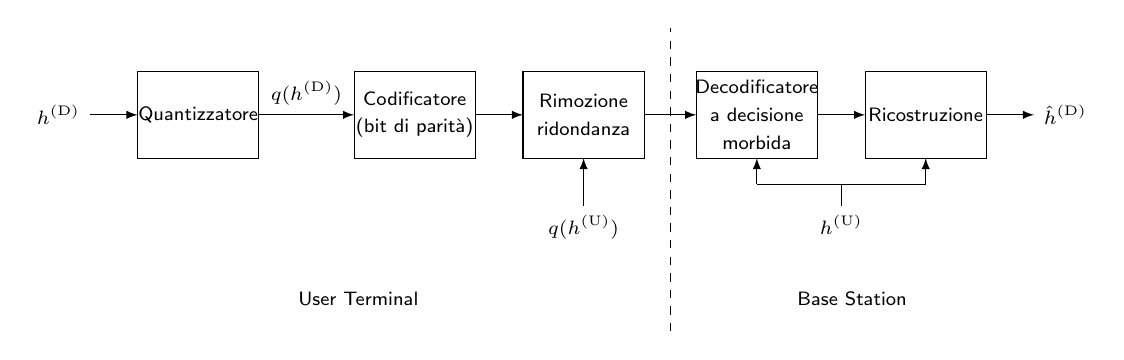
\begin{tikzpicture}[scale=0.55,>=latex]
    \tikzstyle{every node}=[font=\fontsize{6.8}{10}\sffamily]

    % Coding at UT
    \draw[->] (1.1,5) node[left]{\(\bm{h}^\mathrm{(D)}\)} -- (2.2,5);

    \draw (2.2,4) rectangle (5,6)
    node[midway,align=center]{Quantizzatore};

    \draw[->] (5,5) -- (7.2,5)
    node[above,midway]{\(q(\bm{h}^\mathrm{(D)})\)};

    \draw (7.2,4) rectangle (10,6)
    node[midway,align=center]{Codificatore \\ (bit di parità)};

    \draw[->] (10,5) -- (11.1,5);

    \draw (11.1,4) rectangle (13.9,6)
    node[midway,align=center]{Rimozione \\ ridondanza};

    \draw[->] (12.5,2.9) node[below]{\(q(\bm{h}^\mathrm{(U)})\)} -- (12.5,4);

    % Send in Feedback
    \draw[->] (13.9,5) -- (15.1,5);
    \draw[-, dashed] (14.5,0) -- (14.5,7);
    \draw (7.3,0.75) node {User Terminal};
    \draw (18.7,0.75) node {Base Station};

    % Decoding at BS
    \draw (15.1,4) rectangle (17.9,6)
    node[midway,align=center]{Decodificatore \\ a decisione \\ morbida};

    \draw[->] (16.5,3.4) -- (16.5,4);

    \draw[->] (17.9,5) -- (19,5);

    \draw (19,4) rectangle (21.8,6)
    node[midway,align=center]{Ricostruzione};

    \draw[->] (20.4,3.4) -- (20.4,4);

    \draw[-] (16.5,3.4) -- (20.4,3.4);
    \draw[-] (18.45,2.9) node[below]{\(\bm{h}^\mathrm{(U)}\)} -- (18.45,3.4);

    \draw[->] (21.8,5) -- (22.9,5)
    node[right]{\(\hat{\bm{h}}^\mathrm{(D)}\)};
\end{tikzpicture}

    \caption{
        Schema della codifica di sorgente con distorsione per la trasmissione
        del canale di DL in feedback.
    }
    \label{fig:procedure-schema}
\end{figure}
\newline
Il decodificatore a decisione morbida infatti può utilizzare un'informazione a
priori sulla distribuzione delle parole di codice. Questa distribuzione è
ottenuta dalla conoscenza del canale di UL e dalla correlazione di quest'ultimo
con il canale di DL.

